\chapter{Diagramme du cas d'utilisation}


\section{Analyse Et Conception:}
Dans cette partie, nous utilisons la modélisation UML pour représenter les spécifications des
exigences grâce au diagramme de cas d’utilisation, mais aussi pour analyser le domaine avec le
diagramme de classe. Par la suite, nous abordons la conception, d’un point de vue fonctionnel,
technique et graphique. 
\section{Spécifications des exigences: Les cas d’utilisations}
Nous allons répondre aux questions suivantes : Quels sont les utilisateurs du système ? Quelles sont
leurs interactions avec celui-ci ? Il faut donc identifier les différents acteurs ainsi que les cas
d’utilisation c’est-à-dire les différentes fonctionnalités du système. 

\section{Les acteurs:}
\subsection{Admin : }
Une personne en charge de la gestion de la plateforme.
\subsection{Le créateur de contenu :}
Le protagoniste principal sur le site, bénéficiant du privilège de créer un compte, de publier et de gérer Rissala.
\subsection{Guest:}
Dans notre contexte, il s'agit de la personne qui consulte les newsletters et s'abonne au créateur de contenu.

\begin{figure}[p]
    \centering
    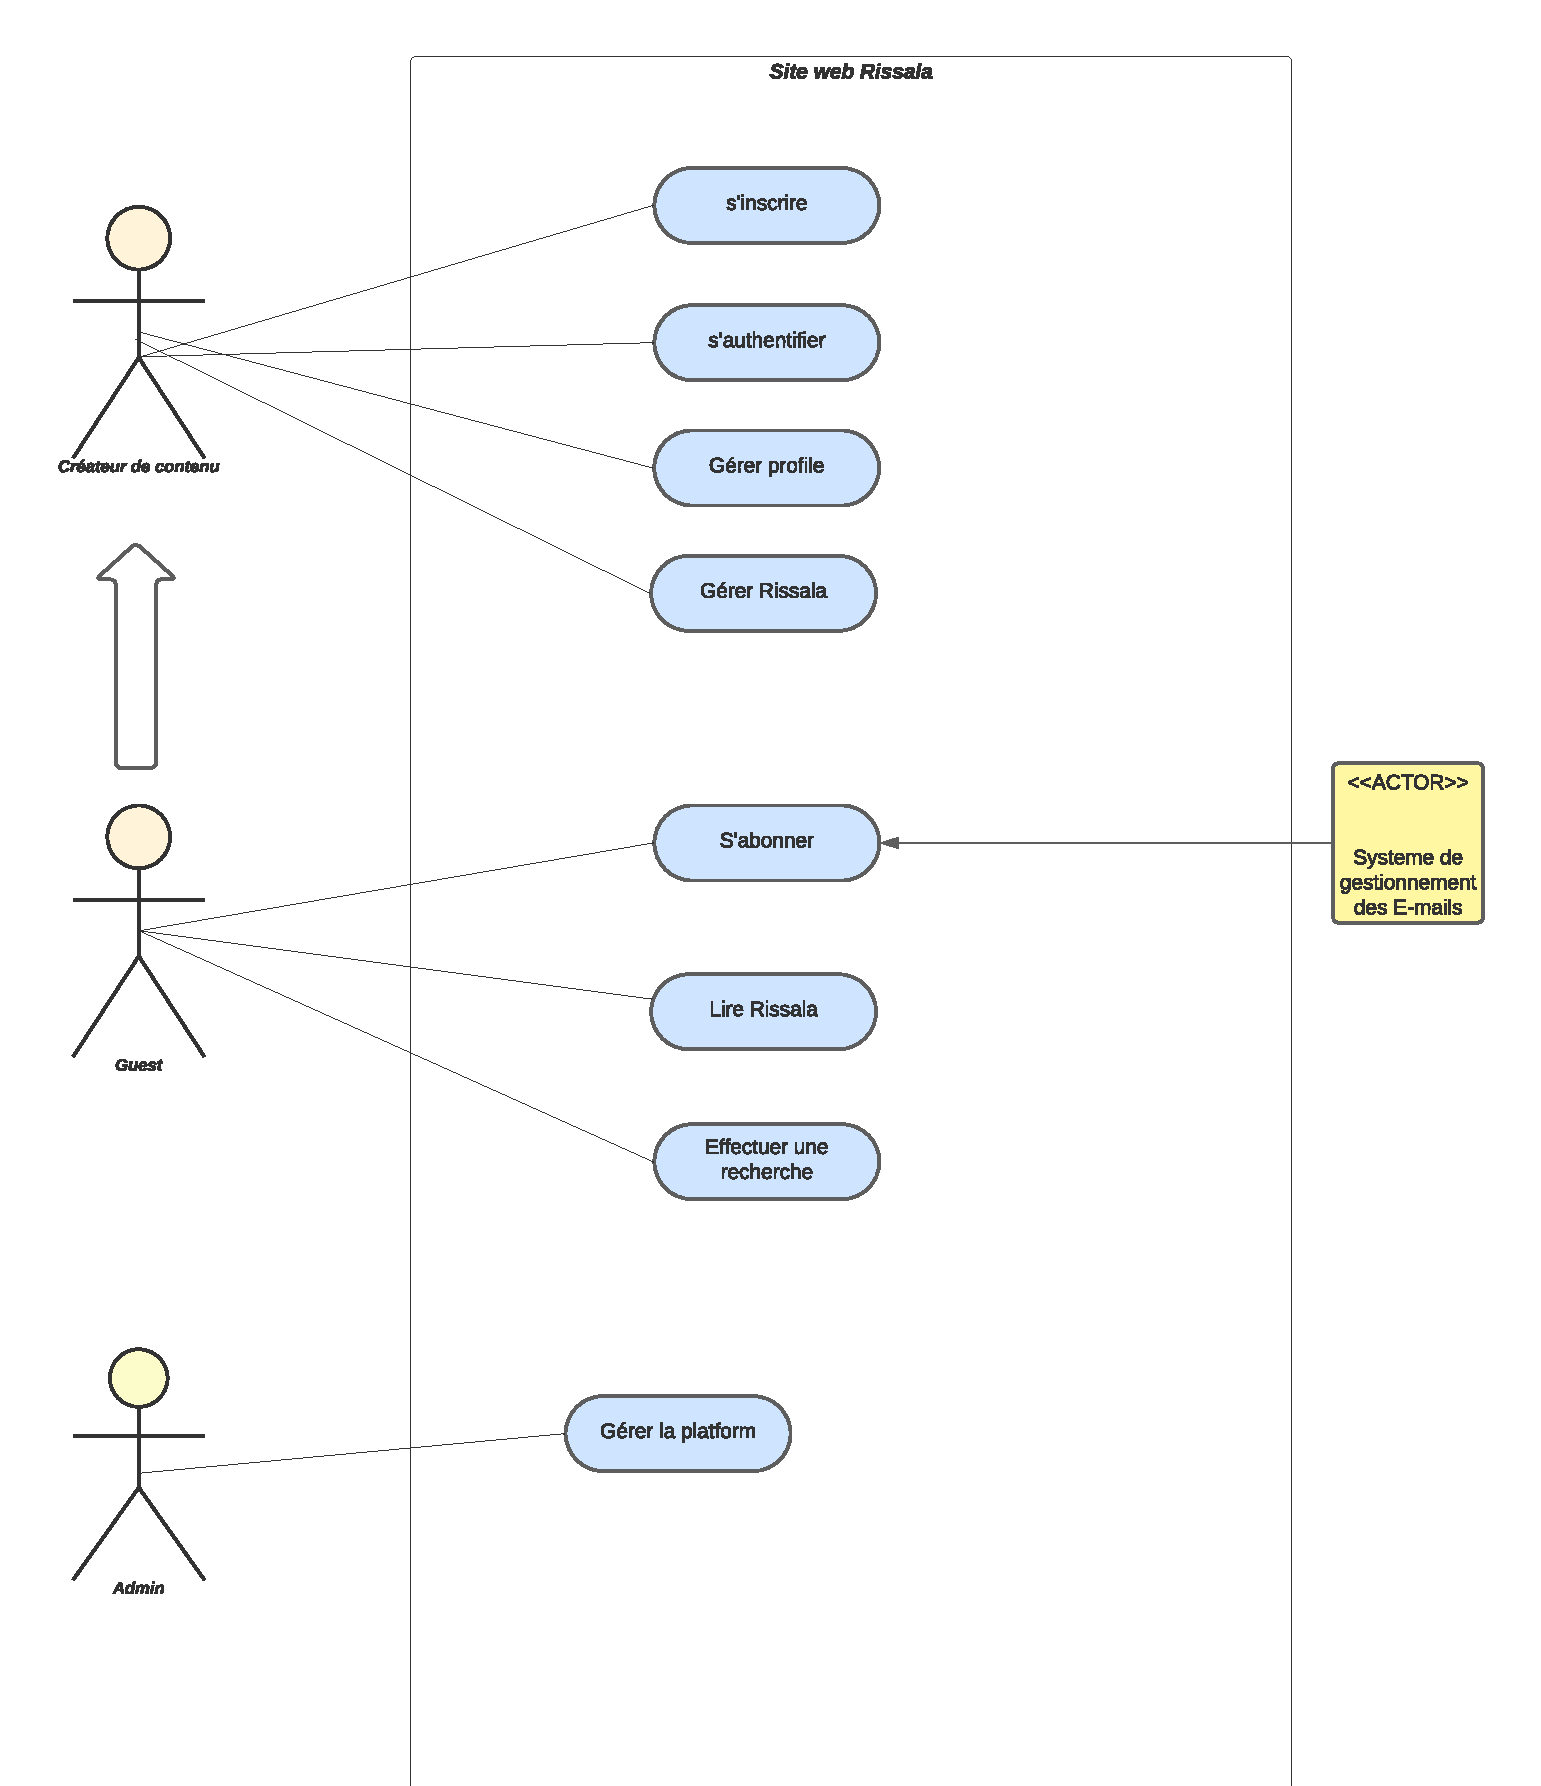
\includegraphics[width=1.\textwidth,height=1.5\textheight,keepaspectratio]{image/Diagramme vierge.pdf}
    \caption{Diagramme du cas d'utilisation n*1}
    \label{fig:diagramme}
\end{figure}